% 0105(본책 23쪽) — 좌표평면 위 반지름 1 사분원, ∠AOB=x 인 반직선 OD(B 는 원 위·A 는 B 의 수선의 발), 접선 x=1 위의 D, C=(1,0), ∠ODC=y. 라벨 O·A·B·C·D·x·y·1(y축)·1(C), 직각 표시(A·C). 스캔 삽화를 TikZ 로 다시 그림. 답(점 B 의 좌표)은 적지 않는다.
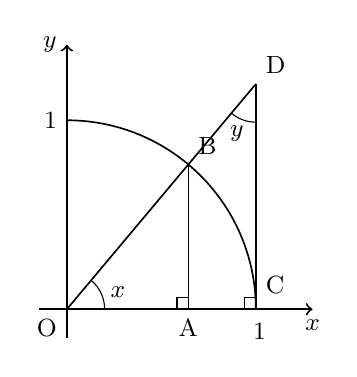
\begin{tikzpicture}[scale=2.4, line width=0.6pt]
  \coordinate (O) at (0,0); \coordinate (B) at (0.6428,0.7660); \coordinate (A) at (0.6428,0); \coordinate (D) at (1,1.1918); \coordinate (C) at (1,0);
  \draw[->, line width=0.7pt] (-0.15,0) -- (1.3,0) node[below, font=\small] {$x$};
  \draw[->, line width=0.7pt] (0,-0.15) -- (0,1.4) node[left, font=\small] {$y$};
  \draw (C) arc[start angle=0, end angle=90, radius=1];
  \draw (O) -- (D);
  \draw (B) -- (A);
  \draw (D) -- (C);
  % 직각 표시
  \draw[line width=0.4pt] (0.6428,0.06) -- (0.5828,0.06) -- (0.5828,0);
  \draw[line width=0.4pt] (1,0.06) -- (0.94,0.06) -- (0.94,0);
  % 각 x(O)·각 y(D)
  \draw[line width=0.4pt] (0.2,0) arc[start angle=0, end angle=50, radius=0.2];
  \node[font=\small] at (0.27,0.09) {$x$};
  \draw[line width=0.4pt] (1,0.99) arc[start angle=-90, end angle=-130, radius=0.2];
  \node[font=\small] at (0.9,0.93) {$y$};
  \node[font=\small, left] at (0,1) {$1$};
  \node[font=\small, below] at (1.02,-0.02) {$1$};
  \node[font=\small, below left] at (O) {O};
  \node[font=\small, below] at (A) {A};
  \node[font=\small, above right] at (B) {B};
  \node[font=\small, above right] at (1,0.03) {C};
  \node[font=\small, above right] at (D) {D};
\end{tikzpicture}
